\documentclass[12pt]{article}

\usepackage{graphicx}
\usepackage{paralist}
\usepackage{amsfonts}
\usepackage{amsmath}
\usepackage{hhline}
\usepackage{booktabs}
\usepackage{multirow}
\usepackage{multicol}
\usepackage{url}

\oddsidemargin -10mm
\evensidemargin -10mm
\textwidth 160mm
\textheight 200mm
\renewcommand\baselinestretch{1.0}

\pagestyle {plain}
\pagenumbering{arabic}

\newcounter{stepnum}

%% Comments

\usepackage{color}

\newif\ifcomments\commentstrue

\ifcomments
\newcommand{\authornote}[3]{\textcolor{#1}{[#3 ---#2]}}
\newcommand{\todo}[1]{\textcolor{red}{[TODO: #1]}}
\else
\newcommand{\authornote}[3]{}
\newcommand{\todo}[1]{}
\fi

\newcommand{\wss}[1]{\authornote{blue}{SS}{#1}}

\title{COMPSCI 2ME3, Assignment 4, Design Specification}
\author{Jie Zhang - zhanj265}

\begin{document}

\maketitle
This Module Interface Specification (MIS) document contains modules, types and
methods for implementing the game \textit{2048}. At the start of each game, the user will be given a 4x4 matrix with two 2's or two 4's or one 2 and one 4. The user can move all tiles in this matrix to up, down, left or right in one round, and tiles with the same number will merge into one when they touch. After each round, if there is still empty space in matrix, there is 90 percent possibility that a random empty space will be filled with 2, and 10 percent possibility that a random empty space will be filled with 4. Throughout this specification document, each tile will be referred as to a space in matrix and a cell(x, y) refers to the position of a tile, where x represents the index of row and y represents the index of column. In addition, row number increases when moving from top to bottom and column number increases when moving from left to right. The game can be launched and play by typing \texttt{make demo} in terminal.


\begin{center}
  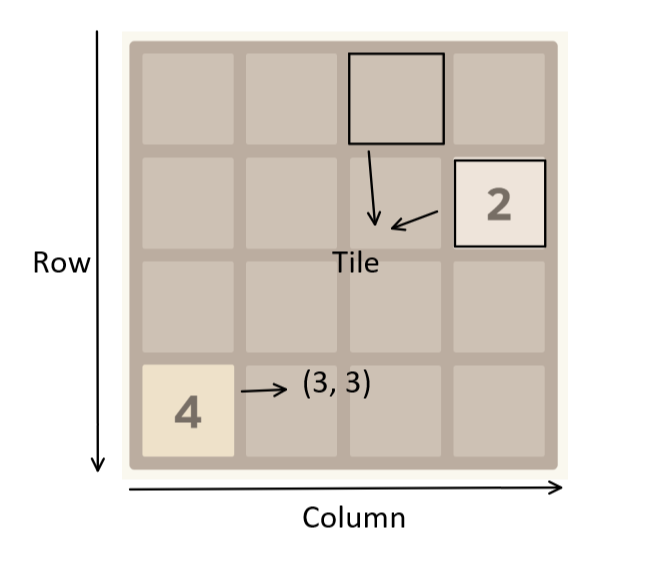
\includegraphics[width=0.6\textwidth]{Game_begin.png}

  The above board visualization is from https://play2048.co/
\end{center}

\newpage

\section{Overview of the design}

This design applies Module View Specification (MVC) design pattern and Singleton design pattern. The MVC components are \textit{GameController} (controller module), \textit{BoardT} (model module), and \textit{TextView} (view module). Singleton pattern is specified and implemented for \textit{GameController} and \textit{TextView}

\bigskip

\noindent An UML diagram is provided below for visualizing the structure of this software architecture

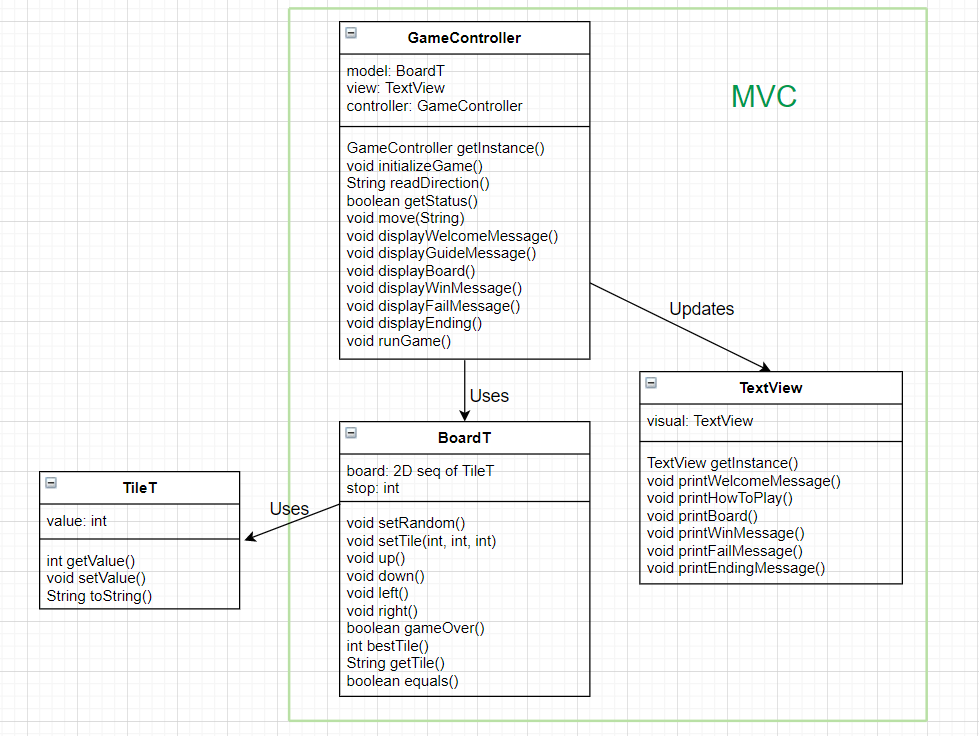
\includegraphics[width=0.9\textwidth]{A4_UML.png}

\medskip
The MVC design pattern is specified and implemented in the following way: the module \textit{BoardT} stores the state of the game board. A view module \textit{TextView} can display the state of the game board using a text-based graphics. The controller \textit{GameController} is responsible for handling input actions and updating the view received by user. 

\medskip

For \textit{GameController} and \textit{TextView}, use the getInstance() method to obtain the abstract object.

\newpage

\subsection*{Likely Changes my design considers:}

\begin{itemize}
  \item Change in the form of view. This specification uses TileT class to store value at each cell in this board. If we want to change the view from text-based to GUI, TileT object can store color based on its value. This class makes future GUI development more convenient.
  \item Change in the size of the game board. 
\end{itemize}

\newpage

\section* {Tile ADT Module}

\subsection*{Template Module}

TileT

\subsection* {Uses}

None

\subsection* {Syntax}

\subsubsection* {Exported Types}

TileT = ?

\subsubsection* {Exported Constant}

None

\subsubsection* {Exported Access Programs}

\begin{tabular}{| l | l | l | l |}
\hline
\textbf{Routine name} & \textbf{In} & \textbf{Out} & \textbf{Exceptions}\\
\hline
TileT & ~ & TileT & \\
\hline
TileT & $\mathbb{N}$ & TileT & \\
\hline
getValue & ~ & $\mathbb{N}$ & \\
\hline
setValue & $\mathbb{N}$ & ~ & \\
\hline
toString & ~ & String & \\
\hline
\end{tabular}

\subsection* {Semantics}

\subsubsection* {State Variables}

value: $\mathbb{N}$

\subsubsection* {State Invariant}

None

\subsubsection* {Assumptions}

\begin{itemize}
  \item The value of TileT is always 0 or the power of 2 (except 1).
\end{itemize}

\subsubsection* {Access Routine Semantics}

TileT():
\begin{itemize}
\item transition: value $:=$ 0
\item output: $out := \mathit{self}$
\item exception: None
\end{itemize}

\noindent TileT(num):
\begin{itemize}
\item transition: value $:=$ num
\item output: $out := \mathit{self}$
\item exception: None
\end{itemize}

\noindent getValue():
\begin{itemize}
\item transition: none
\item output: $out :=$ value
\item exception: None
\end{itemize}

\noindent setValue(num):
\begin{itemize}
\item transition: value $:=$ num
\item output: None
\item exception: None
\end{itemize}

\noindent toString():
\begin{itemize}
\item transition: none
\item output: $out :=$ value.toString()
\item exception: None
\end{itemize}

\newpage

\section* {Board ADT Module}

\subsection*{Template Module}

BoardT

\subsection* {Uses}

TileT

\subsection* {Syntax}

\subsubsection* {Exported Types}

None

\subsubsection* {Exported Constant}

size = 4 \quad // Size of the board 4 x 4

\subsubsection* {Exported Access Programs}

\begin{tabular}{| l | l | l | l |}
\hline
\textbf{Routine name} & \textbf{In} & \textbf{Out} & \textbf{Exceptions}\\
\hline
BoardT & ~ & BoardT & \\
\hline
BoardT & seq of (seq of TileT) & BoardT & \\
\hline
setRandom & ~ & ~ & \\
\hline
setTile & $\mathbb{N}$, $\mathbb{N}$, $\mathbb{N}$ & ~ & IndexOutOfBoundsException\\
\hline
up & ~ & ~ & \\
\hline
down & ~ & ~ & \\
\hline
left & ~ & ~ & \\
\hline
right & ~ & ~ & \\
\hline
gameOver & ~ & $\mathbb{B}$ & \\
\hline
bestTile & ~ & $\mathbb{N}$ & \\
\hline
getTile & $\mathbb{N}$, $\mathbb{N}$ & String & IndexOutOfBoundsException\\
\hline
equals & BoardT & $\mathbb{B}$ & \\
\hline
\end{tabular}

\subsection* {Semantics}

\subsubsection* {State Variables}

board: sequence [size, size] of TileT \\
stop: $\mathbb{N}$ 
\textit{// help to store which tile cannot merge when moving them.}

\subsubsection* {State Invariant}

None

\subsubsection* {Assumptions}

\begin{itemize}
  \item The constructor BoardT is called for each object instance before any other access routine is called for that object. 
  \item Assume there is a random function that generates a random value beteern 0 and 1 (not included 1).
\end{itemize}

\subsubsection* {Design decision}

The coordinates of the board is stored in a 2D sequence. In later specification, board[x][y] and board(x,y) both mean the TileT at row x and column y of the board. Row number increases when moving from top to bottom and column number increases when moving from left to right, and they both start from 0. Since this game is text-based, all empty spaces in board are represented by tiles with value of 0.

\subsubsection* {Access Routine Semantics}

BoardT():
\begin{itemize}
\item transition: \\
      board $:=$ 
      $\langle \begin{array}{c}
      \langle 0, 0, 0, 0 \rangle\\
      \langle 0, 0, 0, 0 \rangle\\
      \langle 0, 0, 0, 0 \rangle\\
      \langle 0, 0, 0, 0 \rangle\\
      \end{array} \rangle$ \\ 
      stop $:=$ 0
\item output: $out := \mathit{self}$
\item exception: None
\end{itemize}

\noindent BoardT($b$):
\begin{itemize}
\item transition: board, stop $:=$ $b$, 0
\item output: $out := \mathit{self}$
\item exception: None
\end{itemize}

\noindent setRandom():
\begin{itemize}
\item transition: board $:=$ board(randomFrom($x, y : \mathbb{N}| 0 <= x < size \land 0 <= y < size \land board[x][y].getValue() = 0: (x, y)$)) $:=$ randomTile()

\textit{// Set a random empty space to be 2 (90 percent possibility) or 4 (10 percent possibility).}
\item output: None
\item exception: None
\end{itemize}

\noindent setTile(x, y, t)
\begin{itemize}
\item transition: board $:=$ board[x][y].setValue(t)
\item output: None
\item exception: ($\neg$ validateCell($x, y) \Rightarrow$ IndexOutOfBoundsException)
\end{itemize}

\noindent up()
\begin{itemize}
\item transition: board $:=$ Move all tiles with positive values in this game board upward until no tiles can move. From top to bottom, when 2 vertically adjacent tiles have the same value, they can merge and the upper one's value become their sum and the lower one's value become 0, which means the cell is empty. A merged tile cannot merge with other tiles in this round again. After this, all tiles with positive values move upward again. In this process, the state variable stop can be used to store which tile cannot merge anymore.
\item output: None
\end{itemize}

\noindent down()
\begin{itemize}
\item transition: board $:=$ Move all tiles with positive values in this game board downward until no tiles can move. From bottom to top, when 2 vertically adjacent tiles have the same value, they can merge and the lower one's value become their sum and the upper one's value become 0, which means the cell is empty. A merged tile cannot merge with other tiles in this round again. After this, all tiles with positive values move downward again. In this process, the state variable stop can be used to store which tile cannot merge anymore.
\item output: None
\end{itemize}

\noindent left()
\begin{itemize}
\item transition: board $:=$ Move all tiles with positive values in this game board to left until no tiles can move. From left to right, when 2 horizontally adjacent tiles have the same value, they can merge and the left one's value become their sum and the right one's value become 0, which means the cell is empty. A merged tile cannot merge with other tiles in this round again. After this, all tiles with positive values move to left again. In this process, the state variable stop can be used to store which tile cannot merge anymore.
\item output: None
\end{itemize}

\noindent up()
\begin{itemize}
\item transition: board $:=$ Move all tiles with positive values in this game board to right until no tiles can move. From right to left, when 2 horizontally adjacent tiles have the same value, they can merge and the right one's value become their sum and the left one's value become 0, which means the cell is empty. A merged tile cannot merge with other tiles in this round again. After this, all tiles with positive values move to right again. In this process, the state variable stop can be used to store which tile cannot merge anymore.
\item output: None
\end{itemize}

\noindent gameOver()
\begin{itemize}
\item output: $out :=$ $\forall$(x, y: $\mathbb{N} | 0 \leq x < size \land 0 \leq y < size \Rightarrow board[x][y] \neq 0$) $\land$ 

$\forall$(x, y: $\mathbb{N} | 0 \leq x < size-1 \land 0 \leq y < size \Rightarrow board[x][y] \neq board[x+1][y]$) $\land$ 

$\forall$(x, y: $\mathbb{N} | 0 \leq x < size \land 0 \leq y < size-1 \Rightarrow board[x][y] \neq board[x][y+1]$)
\item exception: None
\end{itemize}

\noindent bestTile()
\begin{itemize}
\item output: out $:=$ max(\{x, y: $\mathbb{N} | 0 \leq x < size \land 0 \leq y < size: board[x][y].getValue()$\})
\item exception: None
\end{itemize}

\noindent getTile(x, y)
\begin{itemize}
\item output: out $:=$ board[x][y].toString()
\item exception: ($\neg$ validateCell($x, y) \Rightarrow$ IndexOutOfBoundsException)
\end{itemize}

\noindent equals(b)
\begin{itemize}
\item output: out $:=$ $\forall$(x, y: $\mathbb{N} | 0 \leq x < size \land 0 \leq y < size \Rightarrow board[x][y].toString() = b.getTile(x, y)$)
\item exception: None
\end{itemize}


\subsubsection* {Local Functions}

randomFrom: seq of T $\rightarrow$ T

\medskip

\noindent randomFrom(Seq) $\equiv$ Seq[$floor(Seq.size*random())$]

\medskip
\noindent randomTile: void $\rightarrow$ $\mathbb{N}$

\medskip
\noindent randomTile() $\equiv$ ($floor(random()*10)=0 \Rightarrow 4 | True \Rightarrow 2$)

\medskip
\noindent validateCell: $\mathbb{N} \times \mathbb{N} \rightarrow \mathbb{B}$ 

\medskip

\noindent validateCell($x, y$) $\equiv$ $x <$ size $\wedge$ $y <$ size $\wedge$ $x >=$ 0 $\wedge$ $y >=$ 0 

\newpage

\section* {TextView Module}

\subsection* {Module}

\subsection* {Uses}

None

\subsection* {Syntax}

\subsubsection* {Exported Types}

None

\subsubsection* {Exported Constants}

None

\subsubsection* {Exported Access Programs}

\begin{tabular}{| l | l | l | p{6cm} |}
\hline
\textbf{Routine name} & \textbf{In} & \textbf{Out} & \textbf{Exceptions}\\
\hline
getInstance & ~ & TextView &  \\
\hline
printWelcomeMessage & ~ & ~ & \\
\hline
printHowToPlay & ~ & ~ & \\
\hline
printBoard & BoardT & ~ & \\
\hline
printWinMessage & ~ & ~ & \\
\hline
printFailMessage & ~ & ~ & \\
\hline
printEndingMessage & ~ & ~ & \\
\hline
\end{tabular}

\subsection* {Semantics}

\subsection*{Environment Variables}

window: A portion of computer screen to display the game and messages

\subsubsection* {State Variables}

visual: TextView

\subsubsection* {State Invariant}

None

\subsubsection* {Assumptions}

\begin{itemize}
\item The TextView constructor is called for each object instance before any
other access routine is called for that object. The constructor can only be
called once.
\end{itemize}

\subsubsection* {Access Routine Semantics}

\noindent getInstance():
\begin{itemize}
  \item transition: visual $:=$ (visual = null $\Rightarrow$ new TextView())
  \item output: \textit{self}
  \item exception: None
\end{itemize}

\noindent printWelcomeMessage():
\begin{itemize}
\item transition: window $:=$ Displays a welcome message when user first enters the game.
\end{itemize}

\noindent printHowToPlay():
\begin{itemize}
\item transition: window $:=$ Displays a message to teach user how to play this game.
\end{itemize}

\noindent printBoard($board$):
\begin{itemize}
\item transition: window $:=$ Draws the game board onto the screen. Each cell of the board is accessed and printed using the $getTile$ method from $BoardT$. The board[x][y] is displayed in a way such that x is increasing from the top of the screen to the bottom, and y value is increasing from the left to the right of the screen. For example, board[0][0] is displayed at the top-left corner and board[size-1][size-1] is displayed at bottom-right corner. 
\end{itemize}

\noindent printWinMessage():
\begin{itemize}
\item transition: window $:=$ Displays a win message when the user wins the game.
\end{itemize}

\noindent printFailMessage():
\begin{itemize}
\item transition: window $:=$ Displays a fail message when the user fails the game.
\end{itemize}

\noindent printEndingMessage():
\begin{itemize}
\item transition: Prints a ending message after the user exit the game (entered ``e'').
\end{itemize}

\subsubsection*{Local Function:}

TextView: void $\rightarrow$ TextView \\
TextView() $\equiv$ new TextView()

\newpage

\section* {GameController Module}

\subsection* {GameController Module}

\subsection* {Uses}

BoardT, TextView

\subsection* {Syntax}

\subsubsection* {Exported Types}

None

\subsubsection* {Exported Constants}

None

\subsubsection* {Exported Access Programs}

\begin{tabular}{| l | l | l | p{4.7cm} |}
\hline
\textbf{Routine name} & \textbf{In} & \textbf{Out} & \textbf{Exceptions}\\
\hline
getInstance & BoardT, TextView & GameController & ~ \\
\hline
initializeGame & ~ & ~ & ~\\
\hline
readDirection & ~ & String & IllegalArgumentException \\
\hline
getStatus& ~ & $\mathbb{B}$ & ~ \\
\hline
move & String & ~ & ~ \\
\hline
displayWelcomeMessage& ~ & ~ & ~ \\
\hline
displayGuideMessage& ~ & ~ & ~ \\
\hline
displayBoard& ~ & ~ & ~ \\
\hline
displayWinMessage& ~ & ~ & ~ \\
\hline
displayFailMessage& ~ & ~ & ~ \\
\hline
displayEnding& ~ & ~ & ~ \\
\hline
runGame & ~ & ~ & ~ \\
\hline
\end{tabular}

\subsection* {Semantics}

\subsection*{Environment Variables}

keyboard: Scanner(System.in) \qquad \textit{// reading inputs from keyboard}

\subsubsection* {State Variables}

model: BoardT \\
view: TextView \\
controller: GameController

\subsubsection* {State Invariant}

None

\subsubsection* {Assumptions}

\begin{itemize}
\item The GameController constructor is called for each object instance before any other access routine is called for that object.  The constructor can only be called once.
\item Assume that model and view instances are already initialized before calling GameController constructor
\end{itemize}

\subsubsection* {Access Routine Semantics}

getInstance($m$, $v$):
\begin{itemize}
\item transition: controller $:=$ (controller = null $\Rightarrow$ new GameController ($m, v$))
item output: \textit{self}
\item exception: None
\end{itemize}

\noindent initializeGame():
\begin{itemize}
\item transition: model $:=$ sum(\{x, y: $\mathbb{N} | 0 \leq x < size \land 0 \leq y < size \land board[x][y].getValue() = 0: 1\}$) = size*size - 2 $\land$ sum(\{x, y: $\mathbb{N} | 0 \leq x < size \land 0 \leq y < size \land (board[x][y].getValue() = 2 \lor board[x][y].getValue() = 4): 1\}$) = 2

\textit{// Initialize an board with only two values, 2 or 4 randomly, at random positions}
\item output: None
\item exception: None
\end{itemize}

\noindent readDirection()
\begin{itemize}
\item output: $input$ : String, entered from the keyboard by the User
\item exception: $exc$ $:=$ (input $\neq$ ``w'' $\wedge$ input $\neq$ ``s'' $\wedge$ input $\neq$ ``a'' $\wedge$ input $\neq$ ``d'' $\wedge$ input $\neq$ ``e'' $\Rightarrow$ IllegalArgumentException)

\textit{// ``w'', ``s'', ``a'', ``d'' for direction, ``e'' to exit the game}
\end{itemize}

\noindent getStatus():
\begin{itemize}
\item transition: None
\item output: $out$ $:=$ model.gameOver()
\item exception: None
\end{itemize}

\noindent move(dir)
\begin{itemize}
\item transition: (dir = ``w'' $\Rightarrow$ model.up() $|$ dir = ``s'' $\Rightarrow$ model.down() $|$ dir = ``a'' $\Rightarrow$ model.left() $|$ dir = ``d'' $\Rightarrow$ model.right())
\item output: None
\end{itemize}

\noindent displayWelcomeMessage():
\begin{itemize}
\item transition: view $:=$ view.printWelcomeMessage()
\end{itemize}

\noindent displayGuideMessage():
\begin{itemize}
\item transition: view $:=$ view.printHowToPlay()
\end{itemize}

\noindent displayBoard():
\begin{itemize}
\item transition: view $:=$ view.printBoard(model)
\end{itemize}

\noindent displayWinMessage():
\begin{itemize}
\item transition: view $:=$ view.printWinMessage()
\end{itemize}

\noindent displayFailMessage():
\begin{itemize}
\item transition: view $:=$ view.printFailMessage()
\end{itemize}

\noindent displayEnding():
\begin{itemize}
\item transition: view $:=$ view.printEndingMessage()
\end{itemize}

\noindent runGame():
\begin{itemize}
\item transition: operational method for running the game. The game will start with a welcome message, next teaching the user how to play this game, then display the board and let the user enter keyboard input to play the game. Eventually, when the game ends, prompt a win or fail message depending on how this game is ended. If the user does not want to play this game in the middle of the game, he/she can enter "e" to exit. Any unacceptable keyboard input will cause the game to end. When a keyboard input is acceptable (except "e), no matter whether it can cause change to the game board, a 2 or 4 will be placed in an empty space after this round. If there is exception, handle it in your way.
\item output: None
\end{itemize}

\subsubsection*{Local Function:}

GameController: BoardT $\times$ TextView $\rightarrow$ GameController \\
GameController($model, view$) $\equiv$ new GameController($model, view$)

\newpage

\section*{Critique of Design}

\begin{itemize}
\item This specification is consistent on name conventions, ordering of parameters in argument lists, and exception handling.
\item This specification is not essential since some methods are not necessary. For example, all display methods in GameController can be replaced by calling the corresponding methods in view. But they are kept, because the specification wants to highlight the functionality of GameController: connect model and view.
\item This design is not general. The seperation of concerns (MVC) of the program allows user to easily predict how the modules can be used.
\item This design is minimal since no method can have transition of state variables and output at the same time.
\item MVC design pattern makes this program more maintainable. It decomposes this program into three components: model component stores the data and state of the game, view component displays the state of the game to the player, and the controller component handles the inputs given by the player and updates view. This design allows programmers to work in parallel. Moreover, development in one component does not require other components to change at the same time. Because of this, this design achieves high cohesion and low coupling.
\item This design is good at information hiding. All state variables are private, but there are also methods that allow data to be accessed from other modules.
\item The two constructors in BoardT improve the flexibilty of the module. The user can choose to play a regular game board by entering \texttt{make demo} or a board that is customized by him/herself. Moreover, the constructor that receives given board makes the testing for BoardT easilier, since we can predict how the board changes after each method and checks its correctness.
\item The GameController and TextView modules are both designed to be an abstract object, because for the game, only one instance is required to control the action and diaplay corresponding message during runtime. Singleton design pattern is also shown here.
\end{itemize}

\newpage

\section*{Answers to Questions:}

Q1:
\begin{center}
  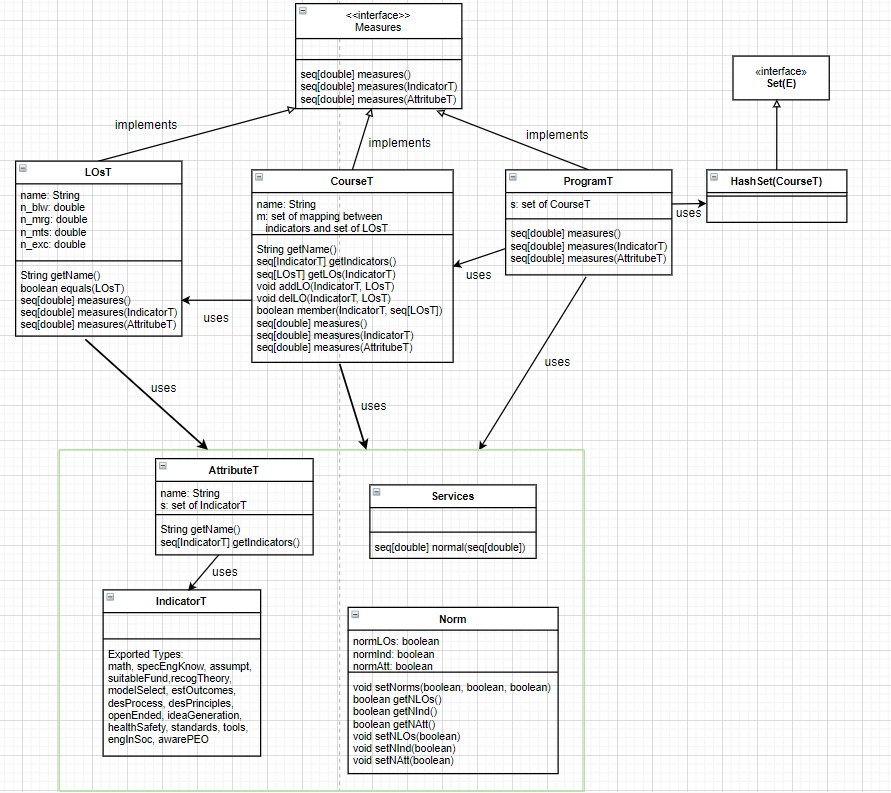
\includegraphics[width=1.2\textwidth]{A3_UML.png}
  Arrows to the green square mean that it uses all 4 modules in the green square.
\end{center}

Q2:
\begin{center}
  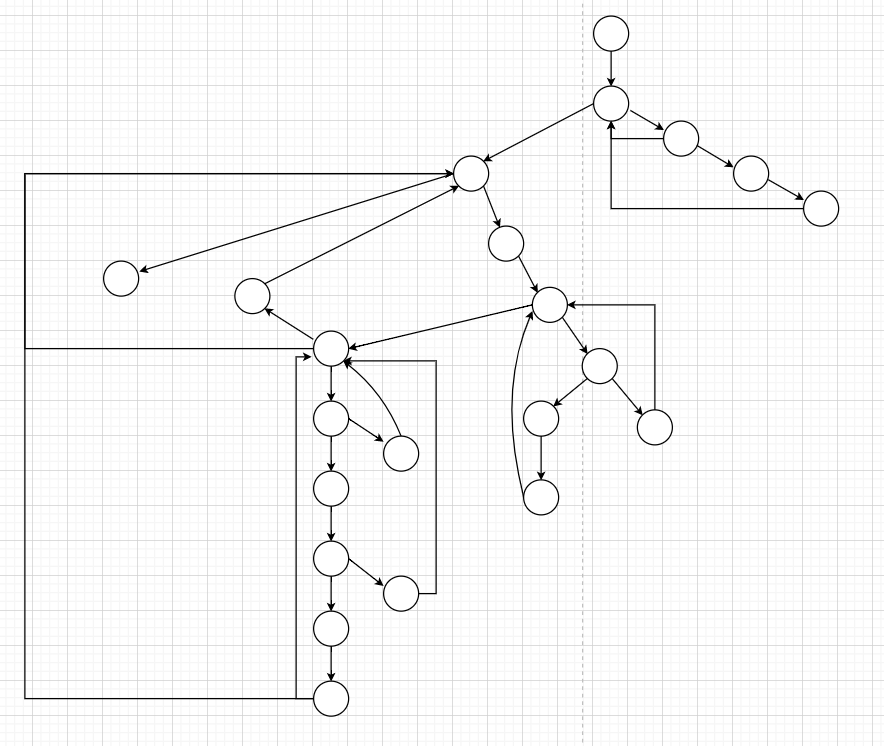
\includegraphics[width=1.0\textwidth]{control_flow2.png}
\end{center}

\end {document}